\Chapter{GTFS-adatbázisok}

A GTFS (\textit{General Transit Feed Specification}) egy olyan nemzetközi szabvánnyá vált formátum, amelyben együtt kezelhetőek a tömegközlekedési menetrendek és a hozzájuk kapcsolódó földrajzi információk \cite{gtfs}, \cite{gtfsspec}. Az ilyen formában megadott adatokat aktuális kutatásokhoz is felhasználják \cite{crowdsending}.

Strukturált, szöveges állományok tartalmazzák az adatokat, amik lényegében egy adatbázis-szerkezetet definiálnak. Ezek CSV-fájlok \texttt{.txt} kiterjesztéssel egy \texttt{.zip} fájlba csomagolva. Mindegyik CSV-fájl egy adatbázistáblának felel meg, a fájl neve pedig a tábla nevét jelenti.

Az egyes táblák és a köztük lévő kapcsolatokat mutatja \aref{fig:gtfs}. ábra. A GTFS-formátum kötelező és opcionális táblákat egyaránt tartalmaz. A kötelező táblák létrehozása és adatokkal való feltöltése mindenképp szükséges a rendszer működéséhez.

%\begin{figure}[htb]
%\centering
%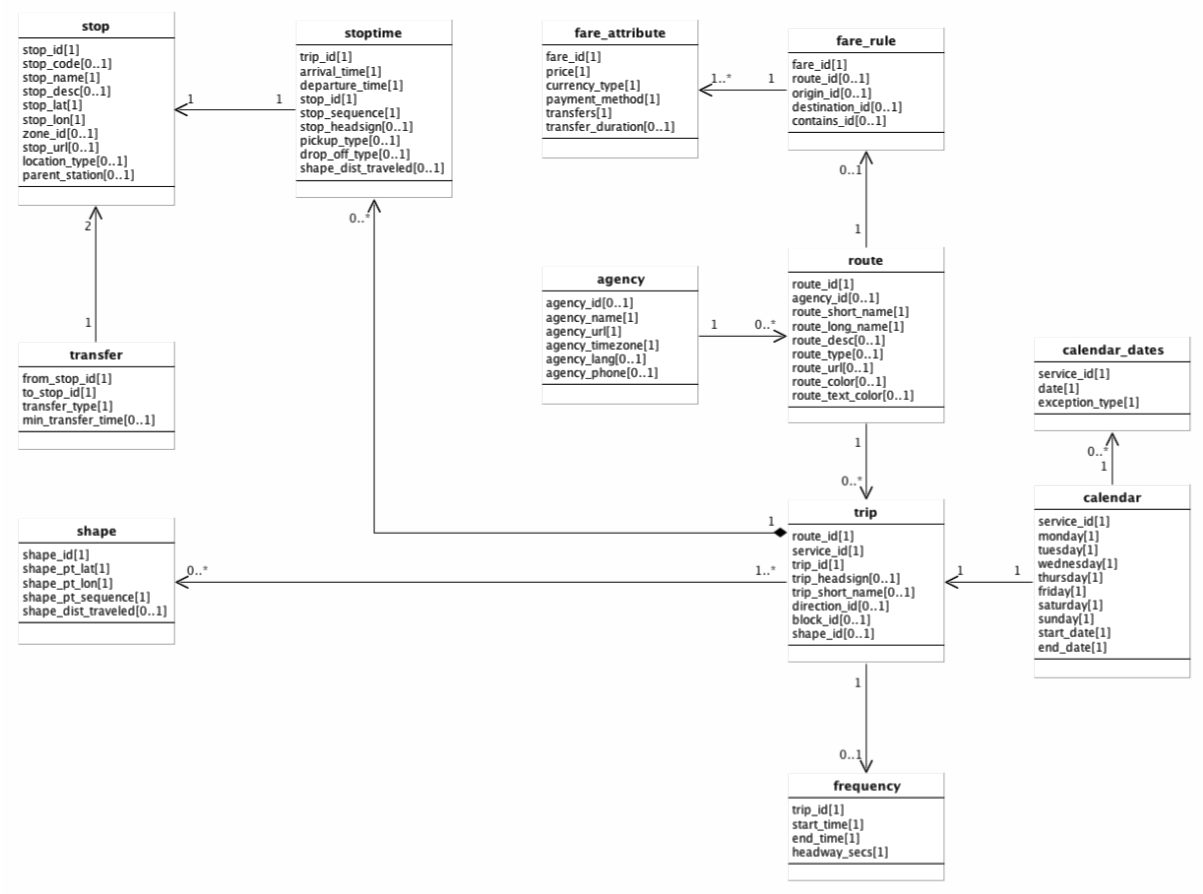
\includegraphics[scale=0.3]{kepek/gtfs_relationships.png}
%\caption{A GTFS-adatbázis tábláinak sémái és a közöttük lévő kapcsolatok.}
%\label{fig:gtfs}
%\end{figure}

\begin{figure}
\centering
\includesvg[width=400pt]{kepek/gtfs}
\caption{A GTFS-adatbázis tábláinak sémái és a közöttük lévő kapcsolatok}
\label{fig:gtfs}
\end{figure}

\Section{Kötelező táblák}

A következő szakaszok a kötelező adatbázistáblákat, azok kötelező és opcionális mezőit mutatják be.

\SubSection{agency}

A tömegközlekedési hálózat üzemeltetőjéről tartalmaz információkat. Több rekord is megadható, ha a járatokat több vállalat is üzemelteti. A route táblában minden viszonylatra meg lehet adni, hogy ki az üzemeltetője.

\medskip

\noindent Kötelező mezők:

\bigskip

\begin{tabular}{|p{3.5cm}|p{10cm}|}
\hline
\texttt{agency\_name} & Az üzemeltető vállalt teljes neve. \\
\hline
\texttt{agency\_url} & A vállalat URL címe. \\
\hline
\texttt{agency\_timezone} & Az időzónát tartalmazza, ahol a vállalat található. \\
\hline
\end{tabular}

\SubSection{routes}

Az aktuálisan elérhető viszonylatokat tartalmazza. Minden viszonylat rendelkezik egy azonosítóval, egy rövid és egy hosszú névvel, valamint a viszonylat típusának az azonosítójával.

\medskip

\noindent Kötelező mezők:

\bigskip

\begin{tabular}{|p{3.5cm}|p{10cm}|}
\hline
\texttt{route\_id} & Elsődleges kulcs, a viszonylat azonosítója. \\
\hline
\texttt{route\_short\_name} & A viszonylat rövid neve (száma). \\
\hline
\texttt{route\_long\_name} & A viszonylat hosszú neve, általában a két végállomást tartalmazza. \\
\hline
\texttt{route\_type} & Típusazonosító, lehetséges értékek:
\begin{itemize}
\item 0: villamos,
\item 1: metró,
\item 2: vasút,
\item 3: autóbusz,
\item 4: komp,
\item 5-7: egyéb járművek.
\end{itemize}
\\
\hline
\end{tabular}

\SubSection{trips}

Ez a tábla tartalmazza a járatokat. Mindegyik egy viszonylathoz tartozik, a \\ \texttt{direction\_id} mezőben adható meg, hogy melyik irányban közlekedik a járat az adott viszonylaton (0 vagy 1 értékkel). Kötelező megadni még egy \texttt{service\_id}-t, ami alapján be lehet azonosítani, hogy a járat mely napokon közlekedik. Egy járathoz tartozhat még egy \texttt{shape} is, amely GPS-koordináták sorozataként a járat útvonalát tartalmazza.

\medskip

\noindent Kötelező mezők:

\bigskip

\begin{tabular}{|p{3cm}|p{10cm}|}
\hline
\texttt{trip\_id} & Elsődleges kulcs, a járat azonosítója. \\
\hline
\texttt{route\_id} & Idegen kulcs, a viszonylatra hivatkozik, amelyen a járat közlekedik. \\
\hline
\texttt{service\_id} & Idegen kulcs, a \texttt{calendar} és a \texttt{calendar\_dates} táblákra hivatkozik, ennek segítségével adható meg, hogy a járat mely napokon közlekedik. \\
\hline
\end{tabular}

\SubSection{stops}

Az egyes megállókat tárolja névvel és földrajzi koordinátákkal.

\medskip

\noindent Kötelező mezők:

\bigskip

\begin{tabular}{|p{3cm}|p{10cm}|}
\hline
\texttt{stop\_id} & Elsődleges kulcs, a megálló azonosítója. \\
\hline
\texttt{stop\_name} & A megálló neve. \\
\hline
\texttt{stop\_lat} & A megálló szélességi fokát tartalmazza. A megadott értéknek WGS 84 szabvány szerintinek kell lenni. \\
\hline
\texttt{stop\_lon} & A megálló hosszúsági fokát tartalmazza. A megadott értéknek WGS 84 szabvány szerintinek kell lenni. \\
\hline
\end{tabular}

\SubSection{stop\_times}

Ez a tábla azt tárolja, hogy egy viszonylat egy járata egy megállóba mikor érkezik meg, mikor indul el onnan, és ez hányadik megállója az adott járatnak.

\medskip

\noindent Kötelező mezők:

\bigskip

\begin{tabular}{|p{3.5cm}|p{9.5cm}|}
\hline
\texttt{stop\_id} & Idegen kulcs, a megálló azonosítója. \\
\hline
\texttt{trip\_id} & Idegen kulcs, a járat azonosítója. \\
\hline
\texttt{arrival\_time} & Érkezési idő, a járat mikor érkezik meg a megállóba. HH:MM:SS formátumban kell megadni. \\
\hline
\texttt{departure\_time} & Indulási idő, a járat mikor indul a megállóból. HH:MM:SS formátumban kell megadni. \\
\hline
\texttt{stop\_sequence} & Azt tartalmazza, hogy hányadik megállója ez a járatnak. Nemnegatív egésznek kell lennie. \\
\hline
\end{tabular}

\SubSection{calendar}

Itt úgynevezett szolgáltatásokat lehet megadni. Egy szolgáltatás azt mondja meg, hogy a járatok, amelyek ehhez a szolgáltatáshoz tartoznak, a hét mely napjain közlekednek. Továbbá meg kell adni egy érvényességi intervallumot is.

\medskip

\noindent Kötelező mezők:

\bigskip

\begin{tabular}{|p{3.5cm}|p{10cm}|}
\hline
\texttt{service\_id} & Elsődleges kulcs, a szolgáltatás azonosítója. \\
\hline
\texttt{monday} & \multirow{7}{10cm}{Azt mondja meg, hogy az adott napon közlekedik-e a járat.
Az értéke lehet:
\begin{itemize}
\item 0, ha az adott napon nem közlekedik, és
\item 1, ha az adott napon közlekedik a járat.
\end{itemize}}
\\
\cline{1-1}
\texttt{tuesday} & \\
\cline{1-1}
\texttt{wednesday} & \\
\cline{1-1}
\texttt{thursday} & \\
\cline{1-1}
\texttt{friday} & \\
\cline{1-1}
\texttt{saturday} & \\
\cline{1-1}
\texttt{sunday} & \\
\hline
\texttt{start\_date} & A szolgáltatás kezdő érvényességi ideje. Az értéket YYYYMMDD formátumban kell megadni. \\
\hline
\texttt{end\_date} & A szolgáltatás érvényességi idejének a vége. Az értéket YYYYMMDD formátumban kell megadni. \\
\hline
\end{tabular}

\Section{Opcionális táblák}

Az adatbázis tartalmaz néhány opcionális táblát. Ezeket a következő szakaszok részletezik.

\SubSection{shapes}

A járatok útvonalát tartalmazza a tábla. Egy útvonal több pontból áll, amelyek ugyanazzal a \texttt{shape\_id}-val vannak ellátva.

\newpage

\noindent Kötelező mezők:

\bigskip

\begin{tabular}{|p{3.7cm}|p{9.8cm}|}
\hline
\texttt{shape\_id} & Az útvonal azonosítója. \\
\hline
\texttt{shape\_pt\_lat} & Az útvonal egy pontjának szélességi fokát tartalmazza. A megadott értéknek WGS 84 szabvány szerintinek kell lenni. \\
\hline
\texttt{shape\_pt\_lon} & Az útvonal egy pontjának hosszúsági fokát tartalmazza. A megadott értéknek WGS 84 szabvány szerintinek kell lenni. \\
\hline
\texttt{shape\_pt\_sequence} & Azt tartalmazza, hogy hányadik pontja ez a útvonalnak. Nemnegatív egésznek kell lennie. \\
\hline
\end{tabular}

\SubSection{calendar\_dates}

A táblának két felhasználási módja van.

Ajánlott: A calendar táblával együttesen, ilyenkor a normál menetrend szerinti kivételes eseteket kell itt megadni.

Alternatív: A calendar táblát kihagyva, csak ezt a táblát használni, az összes szolgáltatást itt megadva. 

\medskip

\noindent Kötelező mezők:

\bigskip

\begin{tabular}{|p{3.5cm}|p{10cm}|}
\hline
\texttt{service\_id} & A szolgáltatás azonosítója. Egy \texttt{(service\_id, date)} páros csak egyszer szerepelhet. \\
\hline
\texttt{date} & Egy dátumot tartalmaz, formátuma: YYYYMMDD. \\
\hline
\texttt{exception\_type} & Lehetséges értékei:
\begin{itemize}
\item 1, ha a szolgáltatást hozzá akarjuk adni az adott naphoz, és
\item 2, ha a szolgáltatást el szeretnék távolítani a megadott napon.
\end{itemize}
Például: ha egy járat közlekedik hétfőnként, de egy ünnep hétfőre esik, így tudjuk megadni, hogy aznap a járat nem közlekedik. \\
\hline
\end{tabular}

\newpage

\SubSection{fare\_attributes}

A különböző viteldíjtípusok megadására szolgál.

\medskip

\noindent Kötelező mezők:

\bigskip

\begin{tabular}{|p{3.5cm}|p{10cm}|}
\hline
\texttt{fare\_id} & A viteldíj azonosítója. \\
\hline
\texttt{price} & A viteldíj ára a \texttt{currency\_type} mezőben meghatározott egységben kifejezve. \\
\hline
\texttt{currency\_type} & A valuta ISO 4217 szabvány szerinti kódja. \\
\hline
\texttt{payment\_method} & Azt határozza meg, hogy a viteldíjat mikor kell kifizetni.
Lehetséges értékei:
\begin{itemize}
\item 0, ha felszálláskor kell fizetni, és
\item 1, ha felszállás előtt kell fizetni.
\end{itemize}
\\
\hline
\texttt{transfers} & Azt specifikálja, hogy hány átszállás lehetséges az adott viteldíjtípussal.
Lehetséges értékei:
\begin{itemize}
\item 0: nem engedélyezett az átszállás
\item 1: egy átszállás engedélyezett
\item 2: két átszállás engedélyezett
\item üres: ha a mező üres, akkor bármennyi átszállás engedélyezett.
\end{itemize}
\\
\hline
\end{tabular}

\SubSection{fare\_rules}

A táblával megadható, hogy a \texttt{fare\_attributes} táblában található viteldíjak hogyan vonatkozzanak az útvonalakra.

\newpage

\noindent Kötelező mező:

\bigskip

\begin{tabular}{|p{3cm}|p{10cm}|}
\hline
\texttt{fare\_id} & Idegen kulcs, a viteldíjat azonosítja. \\
\hline
\end{tabular}

\bigskip

\noindent Opcionális mezők:

\bigskip


% TODO: Az utolsó három jobb oldali mező össze van vonva!

\begin{tabular}{|p{3.5cm}|p{9.5cm}|}
\hline
\texttt{route\_id} & Idegen kulcs, a viszonylat azonosítója. Ha több viszonylathoz is ugyanaz a viteldíj tartozik, akkor minden egyes viszonylatot külön rekordként kell felvinni a táblában. \\
\hline
\texttt{origin\_id} & \multirow{3}{10cm}{Idegen kulcsok, a \texttt{stops} tábla \texttt{zone\_id} mezőire hivatkozhatnak.} \\
\cline{1-1}
\texttt{destination\_id} & \\
\cline{1-1}
\texttt{contains\_id} & \\
\hline
\end{tabular}

\SubSection{frequencies}

Ha egy járat szerepel ebben a táblában, akkor az útvonaltervező figyelmen kívül hagyja a \texttt{stop\_times} tábla \texttt{arrival\_time} és \texttt{departure\_time} mezőjét. Ehelyett a  \texttt{stop\_\-times} tábla a megállók sorrendjét és az egyes megállók közötti időkülönbséget határozza meg.

\medskip

\noindent Kötelező mezők:

\bigskip

\begin{tabular}{|p{3cm}|p{10cm}|}
\hline
\texttt{trip\_id} & Idegen kulcs, egy járatra hivatkozik. \\
\hline
\texttt{start\_time} & Az az időpont, amikor az első jármű elhagyja a járat első megállóját. \\
\hline
\texttt{end\_time} & Az az időpont, amikor a járat egy másik gyakoriságra vált. \\
\hline
\texttt{headway\_secs} & Másodpercekben kifejezve, hogy a \texttt{start\_time} és az \texttt{end\_time} mezők által meghatározott időintervallumon belül mennyi idő telik el két indulás között ugyanabból a megállóból. \\
\hline
\end{tabular}

\SubSection{transfers}

Útvonaltervezők általában az átszállási pontokat az egyes viszonylatok megállóinak a távolságai alapján számítják ki. Az esetlegesen kétértelmű megállópárok egyértelműsítésére vagy egy konkrét csatlakozási lehetőség megadására szolgál ez a tábla.

\newpage

\noindent Kötelező mezők:

\bigskip

\begin{tabular}{|p{3cm}|p{10cm}|}
\hline
\texttt{from\_stop\_id} & Idegen kulcs. Egy megálló azonosítóját tartalmazza, ahol a viszonylatok közti kapcsolat kezdődik.  \\
\hline
\texttt{to\_stop\_id} & Idegen kulcs. Egy megálló azonosítóját tartalmazza, ahol a viszonylatok közti kapcsolat végződik. \\
\hline
\texttt{transfer\_type} & A két megálló \texttt{(from\_stop\_id, to\_stop\_id)} közti kapcsolat típusát adja meg.
Lehetséges értékek:
\begin{itemize}
\item 0 vagy üres: Ajánlott átszállási pont a viszonylatok között.
\item 1: Időzített átszállási pont két viszonylat között. Az induló jármű megvárja az érkezőt, elegendő időt biztosítva az utasok számára az átszálláshoz.
\item 2: Az átszállás biztosításához bizonyos idő szükséges. Az ehhez szükséges időt a min\_transfer\_time mező tartalmazza.
\item 3: Az adott helyen átszállás nem lehetséges a viszonylatok között.
\end{itemize}
\\
\hline
\end{tabular}

\SubSection{feed\_info}

Ez a tábla az adatokat publikáló szervezetről tartalmaz információkat. Abban az esetben van fontosabb szerepe, ha a tömegközlekedési hálózat üzemeltetője és az adatok publikálója nem ugyanaz a szervezet.

\medskip

\noindent Kötelező mezők:

\bigskip

\begin{tabular}{|p{4.5cm}|p{8.5cm}|}
\hline
\texttt{feed\_publisher\_name} & Az adatokat szolgáltató szervezet teljes neve. Általában megegyezik az \texttt{agency} tábla \texttt{agency\_name} mezőével. \\
\hline
\texttt{feed\_publisher\_url} & Az adatokat szolgáltató szervezet URL-címe. Általában megegyzik az \texttt{agency} tábla \texttt{agency\_url} mezőével. \\
\hline
\texttt{feed\_lang} & A szövegek alapértelmezett nyelvének IETF BCP 47 nyelvkódját tartalmazza. \\
\hline
\end{tabular}

\Section{GTFSDB}

A nyers GTFS-adatok feldolgozásához először a Google TransitFeed modulját kezdtem el használni. Ennek segítségével a memóriába be tudtam tölteni az adatokat, amiknek a lekérdezésére és a módosítására is lehetőség volt. Azonban hamar arra a következtetésre jutottam, hogy ez számomra nem lesz tökéletesen megfelelő, hiszen én mindenféleképpen adatbázisban szeretném tárolni az adatokat. A Google által kifejlesztett API segítségével is lehet az adatokat lekérdezni és módosítani, azonban úgy gondoltam, hogy az adatbázisban történő tárolással több és jobb lehetőség nyílik erre. A másik ok, amiért erre a következtetésre jutottam, hogy az adatokat ezáltal perzisztensen tudom tárolni.

Elkezdtem ilyen megoldás után kutakodni, így találtam rá az OpenTransitTools GTFSDB nevű könyvtárára. A projekt célja, hogy a GTFS-adatokat programozható kontextusba helyezze szoftverfejlesztők számára. Ennek igen nagy létjogosultsága van, hiszen a GTFS-adatokkal foglalkozó alkalmazások készítésénél általában az első lépés a nyers adatok lekérdezhetővé, feldolgozhatóvá tétele. A GTFSDB könyvtár segítségével PostgreSQL, Oracle, MySQL és SQLite adatbázisokat hozhatunk létre a nyers adatokból. A projekt forráskódja elérhető GitHubon:

\begin{center}
\url{https://github.com/OpenTransitTools/gtfsdb}
\end{center}

Az adatbázis létrehozása és feltöltése a \texttt{database\_load} függvény meghívásával történik. Paraméterként meg kell adni a GTFS-adatokat tartalmazó \texttt{.zip} fájlt, illetve a létrehozni kívánt adatbázisfájl helyét, nevét és típusát. Ezt lefuttatva létrejönnek a táblák és feltöltődnek adatokkal. Ez után már SQLAlchemy segítségével könnyedén lekérdezhetővé válnak az adatok.

\begin{python}
path = resource_filename('gtfsdb', 'zips')
gtfs_file = 'file:///{0}'.format(os.path.join(path, 'mvkzrt.zip'))
basedir = os.path.abspath(os.path.dirname(__file__))
url = 'sqlite:///' + os.path.join(basedir, 'mvk.db')
db = database_load(gtfs_file, url=url)
\end{python}

A GTFSDB-t Python 2.7-es verzióval ajánlott használni, így először én is azzal próbáltam. Ezáltal viszont a következő problémába ütköztem bele. Az adatbázis feltöltése közben hiba keletkezett, nem sikerült az ékezeteket tartalmazó szövegek feldolgozása. Témavezetőm azt tanácsolta, hogy próbáljam meg a Python hármas verziójával lefuttatni a kódot, és akkor valószínűleg az ékezetes betűkből adódó karakterkódolási hiba meg fog szűnni. Ahhoz, hogy a GTDSDB működjön Python 3-mal, ahhoz a forráskódjában néhány sort át kellett írni. A következőkben ezeket a változtatásokat ismertetem.

\newpage

\noindent \texttt{gtfsdb/config.py}

1. sor:
\begin{python}
-from ConfigParser import ConfigParser
+from configparser import ConfigParser
\end{python}

\bigskip

\bigskip

\noindent \texttt{gtfsdb/model/base.py}

33. sor:
\begin{python}
-except Exception, e:
+except Exception as e: 
\end{python}

158. sor:
\begin{python}
-if isinstance(v, basestring):
+if isinstance(v, str):
\end{python}

171. sor:
\begin{python}
-except Exception, e:
+except Exception as e:
\end{python}

\bigskip

\noindent \texttt{gtfsdb/model/db.py}

82. sor:
\begin{python}
-except Exception, e:
+except Exception as e:
\end{python}

\bigskip

\noindent \texttt{gtfsdb/model/gtfs.py}

6. sor:
\begin{python}
-from urllib import urlretrieve
+from urllib.request import urlretrieve
\end{python}

53. sor:
\begin{python}
-except Exception, e:
+except Exception as e:
\end{python}

\newpage

\noindent \texttt{gtfsdb/model/route\_stop.py}

260. sor:
\begin{python}
-print unique_stops
+print(unique_stops)
\end{python}

\bigskip

\noindent \texttt{gtfsdb/model/stop\_time.py}

75. sor:
\begin{python}
-except Exception, e:
+except Exception as e:
\end{python}


Ezekkel a változtatásokkal, Python 3 alatt, sikeresen lefutott a \texttt{database\_load} függvény ékezetes karaktereket tartalmazó forrásfájlok esetén is.
